\documentclass{sigchi}

% Use this section to set the ACM copyright statement (e.g. for
% preprints).  Consult the conference website for the camera-ready
% copyright statement.

% Copyright
\CopyrightYear{2016}
%\setcopyright{acmcopyright}
\setcopyright{acmlicensed}
%\setcopyright{rightsretained}
%\setcopyright{usgov}
%\setcopyright{usgovmixed}
%\setcopyright{cagov}
%\setcopyright{cagovmixed}
% DOI
\doi{http://dx.doi.org/10.475/123_4}
% ISBN
\isbn{123-4567-24-567/08/06}
%Conference
\conferenceinfo{CHI'16,}{May 07--12, 2016, San Jose, CA, USA}
%Price
\acmPrice{\$15.00}

% Use this command to override the default ACM copyright statement
% (e.g. for preprints).  Consult the conference website for the
% camera-ready copyright statement.

%% HOW TO OVERRIDE THE DEFAULT COPYRIGHT STRIP --
%% Please note you need to make sure the copy for your specific
%% license is used here!
% \toappear{
% Permission to make digital or hard copies of all or part of this work
% for personal or classroom use is granted without fee provided that
% copies are not made or distributed for profit or commercial advantage
% and that copies bear this notice and the full citation on the first
% page. Copyrights for components of this work owned by others than ACM
% must be honored. Abstracting with credit is permitted. To copy
% otherwise, or republish, to post on servers or to redistribute to
% lists, requires prior specific permission and/or a fee. Request
% permissions from \href{mailto:Permissions@acm.org}{Permissions@acm.org}. \\
% \emph{CHI '16},  May 07--12, 2016, San Jose, CA, USA \\
% ACM xxx-x-xxxx-xxxx-x/xx/xx\ldots \$15.00 \\
% DOI: \url{http://dx.doi.org/xx.xxxx/xxxxxxx.xxxxxxx}
% }

% Arabic page numbers for submission.  Remove this line to eliminate
% page numbers for the camera ready copy
% \pagenumbering{arabic}

% Load basic packages
\usepackage{balance}       % to better equalize the last page
\usepackage{graphics}      % for EPS, load graphicx instead 
\usepackage[T1]{fontenc}   % for umlauts and other diaeresis
\usepackage{txfonts}
\usepackage{mathptmx}
\usepackage[pdflang={en-US},pdftex]{hyperref}
\usepackage{color}
\usepackage{booktabs}
\usepackage{textcomp}

% Some optional stuff you might like/need.
\usepackage{microtype}        % Improved Tracking and Kerning
% \usepackage[all]{hypcap}    % Fixes bug in hyperref caption linking
\usepackage{ccicons}          % Cite your images correctly!
% \usepackage[utf8]{inputenc} % for a UTF8 editor only

% If you want to use todo notes, marginpars etc. during creation of
% your draft document, you have to enable the "chi_draft" option for
% the document class. To do this, change the very first line to:
% "\documentclass[chi_draft]{sigchi}". You can then place todo notes
% by using the "\todo{...}"  command. Make sure to disable the draft
% option again before submitting your final document.
\usepackage{todonotes}


% Custom Stuff
\graphicspath{{figures/}{pictures/}{images/}{./}}
\newcommand{\figref}[1]{\hyperref[#1]{Figure~\ref*{#1}}}
\usepackage{xspace}
\newcommand{\ie}{{i.e.}\xspace}
\newcommand{\eg}{{e.g.,}\xspace}
\newcommand{\cf}{{c.f.}\xspace}
\newcommand{\ea}{{et~al.}\xspace}
\newcommand{\aka}{{a.k.a.}\xspace}
\newcommand{\etc}{{etc.}\xspace}
\hyphenation{LayerCake}

\usepackage{subcaption}
\usepackage{amsmath}
\usepackage{hyperref}


% Paper metadata (use plain text, for PDF inclusion and later
% re-using, if desired).  Use \emtpyauthor when submitting for review
% so you remain anonymous.
\def\plaintitle{Tree-like Uncertainty Maps}
\def\plainauthor{Correll, Moritz, Heer}
\def\emptyauthor{}
\def\plainkeywords{Uncertainty Visualization; Color Perception; Thematic Maps; Semiotics.}
\def\plaingeneralterms{Uncertainty Visualization, Color Perception}

% llt: Define a global style for URLs, rather that the default one
\makeatletter
\def\url@leostyle{%
  \@ifundefined{selectfont}{
    \def\UrlFont{\sf}
  }{
    \def\UrlFont{\small\bf\ttfamily}
  }}
\makeatother
\urlstyle{leo}

% To make various LaTeX processors do the right thing with page size.
\def\pprw{8.5in}
\def\pprh{11in}
\special{papersize=\pprw,\pprh}
\setlength{\paperwidth}{\pprw}
\setlength{\paperheight}{\pprh}
\setlength{\pdfpagewidth}{\pprw}
\setlength{\pdfpageheight}{\pprh}

% Make sure hyperref comes last of your loaded packages, to give it a
% fighting chance of not being over-written, since its job is to
% redefine many LaTeX commands.
\definecolor{linkColor}{RGB}{6,125,233}
\hypersetup{%
  pdftitle={\plaintitle},
% Use \plainauthor for final version.
%  pdfauthor={\plainauthor},
  pdfauthor={\emptyauthor},
  pdfkeywords={\plainkeywords},
  pdfdisplaydoctitle=true, % For Accessibility
  bookmarksnumbered,
  pdfstartview={FitH},
  colorlinks,
  citecolor=black,
  filecolor=black,
  linkcolor=black,
  urlcolor=linkColor,
  breaklinks=true,
  hypertexnames=false
}

% create a shortcut to typeset table headings
% \newcommand\tabhead[1]{\small\textbf{#1}}

% End of preamble. Here it comes the document.
\begin{document}

\title{\plaintitle}

%Figure list:
% Vsum vs. traditional 2D heatmap vs. juxtaposed maps
% Chart of color bins w/r/t CIELAB threshold, with iconic maps at intervals
% Process figure
% Real examples with different color maps




\newcommand{\teaserFig}{
  \teaser{
		\centering
		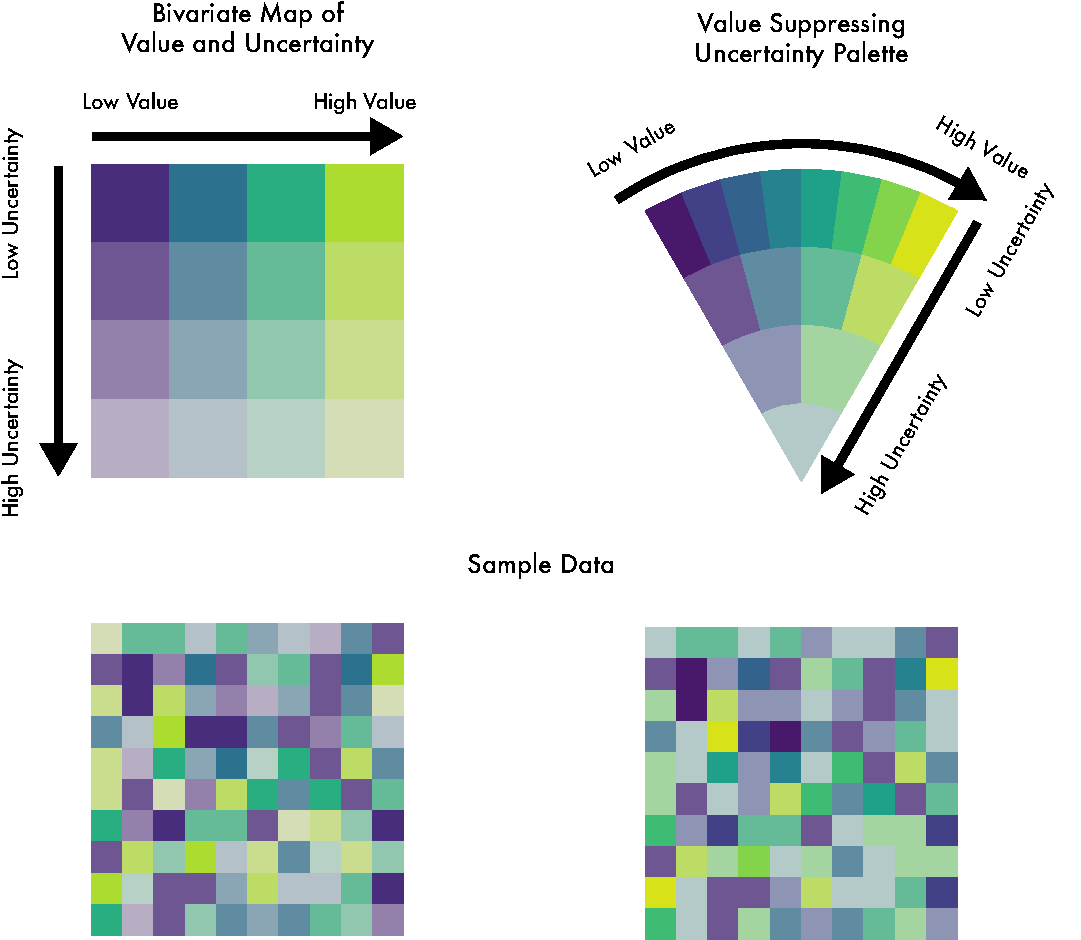
\includegraphics[width=0.9\textwidth]{example.pdf}
		\caption{Lookit! Lookit!}
		\label{fig:teaser}
	}
}

\newcommand{\exampleFig}{
\begin{figure}
	\centering
	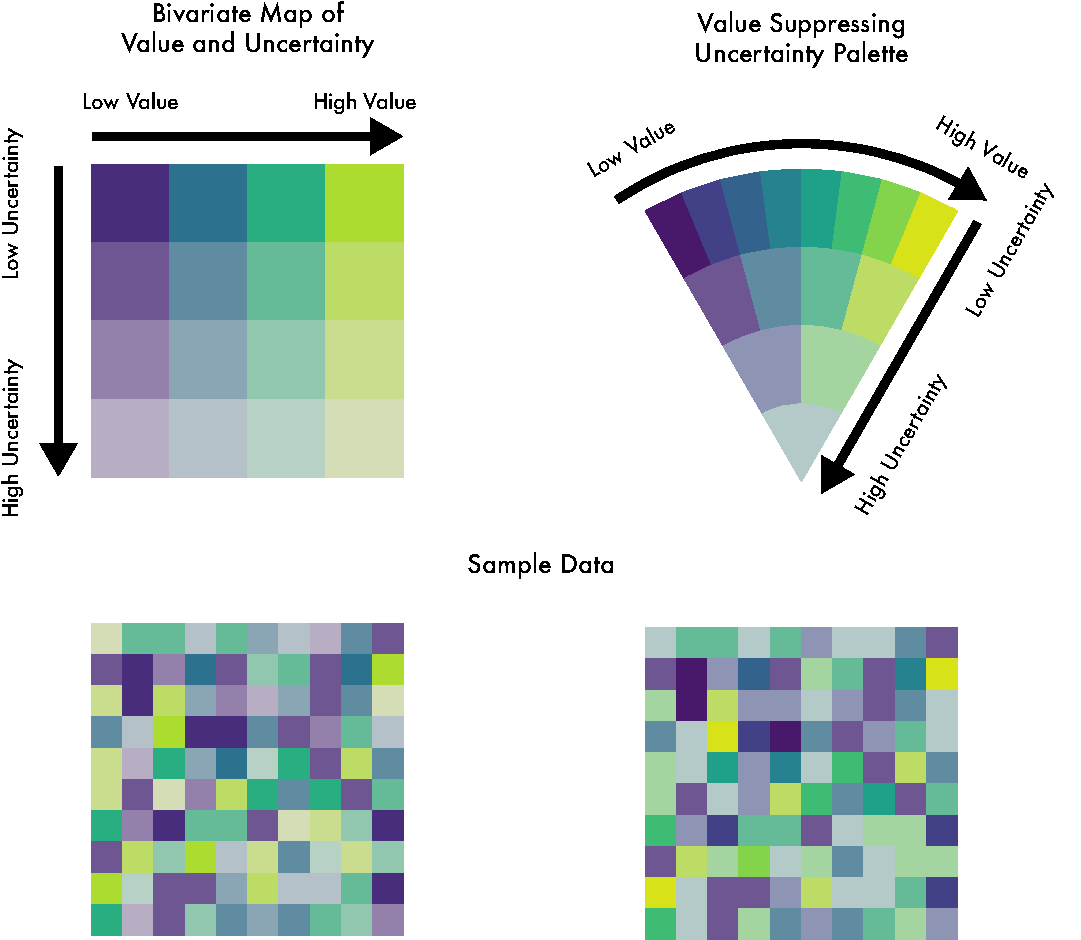
\includegraphics[width=0.9\columnwidth]{example.pdf}
	\caption{A comparison between a standard bivariate map and a VSUM. Both use the same visual channels to encode value (position along the Viridis color map) and uncertainty (lightness and saturation), and have an equal standard of perceptual discriminability (at least 18 units of distance in CIELAB color space between colors). However, highly uncertain values result in colors that are very close together in the bivariate case, meaning the full bivariate map is only 9 bins under these constraints--- a 4x4 map would result in colors that are perceptually too close together. By contrast, the VSUM intentionally reduces bins when uncertainty is high, eventually aliasing all highly uncertain values to the same color. This decision affords more distinct colors in other regions of the map, and so an increase in overall bins to 15. The resulting map suppresses the value of uncertain data, but increases the discriminability of highly certain data.}
	\label{fig:example}
\end{figure}

}

\numberofauthors{3}
\author{%
  \alignauthor{Leave Authors Anonymous\\
    \affaddr{for Submission}\\
    \affaddr{City, Country}\\
    \email{e-mail address}}\\
  \alignauthor{Leave Authors Anonymous\\
    \affaddr{for Submission}\\
    \affaddr{City, Country}\\
    \email{e-mail address}}\\
  \alignauthor{Leave Authors Anonymous\\
    \affaddr{for Submission}\\
    \affaddr{City, Country}\\
    \email{e-mail address}}\\
}

\maketitle

\begin{abstract}
  Uncertainty is a vital concern in many datasets. Visualizations often use bivariate mappings to encode value and uncertainty simultaneously. Due to interference between visual channels, these bivariate maps are limited in discriminability. We contribute Value-Suppressing Uncertainty Maps (VSUMs), an encoding technique that intentionally impairs value discrimination as uncertainty increases. In contrast to traditional bivariate maps, VSUMs alias values when uncertainty is high: expected values with lower uncertainty can be more precisely compared, whereas similar values with higher uncertainty are made harder to differentiate. By making informed binning decisions, VSUMs seek to better use the limited budget of discriminable marks in bivariate maps, and dissuade analysts from making decisions based on data with high uncertainty. We demonstrate several examples of VSUMs and present a crowdsourced evaluation showing that, compared to traditional bivariate maps, VSUMs bias analysts to more heavily weight uncertainty information in decision-making tasks.
\end{abstract}

\category{H.5.0.}{Information Interfaces and Presentation
  (e.g. HCI)}{General}

\keywords{\plainkeywords}

%

\section{Introduction}
Uncertainty is an inescapable component of collecting, presenting, and using data. A common goal in the communication of uncertainty is promoting \emph{uncertainty-aware decisions}: the audience should be aware of the risks and rewards of certain decisions, modulate their confidence in their conclusions, and perhaps refrain from making a decision at all if there is too much uncertainty.  A way that designers can contribute to this goal is by ensuring that uncertainty information is \emph{well-integrated} with the rest of the data. That is, it should be difficult to discount or ignore the uncertainty in a dataset.

Simultaneous presentation of uncertainty and value necessitates the construction of a bivariate map\,---\,a relation, in terms of visual variables, between 2-tuples $(\text{value}, \text{uncertainty})$ and mark properties. The design of bivariate maps is difficult and, due to the interference and interplay between different visual variables, often leads to maps with few discriminable categories.

In this paper, we contribute \textbf{Value-Suppressing Uncertainty Palettes} (VSUPs) for integrating data and uncertainty information in visualizations.
VSUP intentionally alias together data values with high uncertainty, affording greater discriminability as uncertainty decreases. If traditional bivariate maps are a two-dimensional square, with differing outputs for each combination of value and uncertainty, VSUP can be thought of as arcs: as uncertainty increases, values are mapped to smaller and smaller sets of outputs, culminating in a singularity where all inputs are mapped to an identical, highly uncertain mark regardless of their data value. \figref{fig:example} shows examples of both a more traditional bivariate map and a VSUP.

We describe the motivations behind the use of VSUPs, examples of their utility for decision-making under uncertainty, and assess VSUPs in a crowdsourced experiment. Our experimental results indicate that VSUPs create close integration between uncertainty and data, promoting rapid but cautious decision-making.

\exampleFig
\section{Related Work}

% What this section needs to do:
% State of the art in uncertainty vis, with heavy emphasis on MacEachren & co.
% Bivariate maps are hard!
% Binning colormaps is de rigueur
% The variables we'd want to use for uncertainty (like value or alpha or size) mess with color discriminability

Despite the acknowledged importance of uncertainty in understanding data, explicit representations of uncertainty are often missing from visualizations~\cite{boukhelifa2009uncertainty}. This is partially due to the complexity of uncertainty as a concept. In typologies from Thomson \ea~\cite{thomson2005typology} and Buttenfield \& Beard~\cite{buttenfield1994graphical}, the authors note that many, occasionally contradictory, concepts can fall under the category of ``uncertainty,'' including data quality, sampling error, credibility, and provenance.

There are many methods for visualizing uncertainty. MacEachren et al. ~\cite{maceachren1992visualizing} presents a theoretical survey of uncertainty visualization generally. Relevant to our domain of heatmaps and thematic maps is work in GIS and cartography; for a survey of uncertainty visualization techniques in GIS, see Kinkeldey et al. \cite{kinkeldey2014assess,kinkeldey2017evaluating}. Yet, despite these wide variety of methods, to our knowledge, there are no established standards for visualizing uncertainty in heatmaps.

Reviewing the state of the art in uncertainty visualization in the field, Greithe \ea~\cite{griethe2006visualization} and Brodlie \ea~\cite{brodlie2012review} present lists of potential techniques for conveying uncertainty in concert with data. Some of these options (interaction, animation, and sonification) are not applicable for static charts; even for dynamic charts, many users do not interact with charts in sufficient detail to recover uncertainty information~\cite{nyt2016}. While we acknowledge the potential utility of these techniques in uncertainty visualization (for instance, the animation used to convey sampling error in Hullman \ea's Hypothetical Outcome Plots~\cite{hullman2015hypothetical}), we limit the scope of our discussion to techniques which center on static charts.

\subsection{Visual Variables for Uncertainty}

% 1d uvis: olston2002visualizing, wickham201140, neyman1937outline

One challenge to conveying uncertainty information is that the decision to explicitly encode uncertainty increases the dimensionality of the data, and so requires the use of (at least one) additional visual channel ~\cite{brodlie2012review}. Uncertainty therefore inherently increases the visual complexity of a visualization. When the data are already complex to convey, and many of the more common or accurate visual variables are in use, allocating an additional dimension is non-trivial. As the number of dimensions increases, finding visual variables that are both perceptually accurate (in either estimation of quantity or discrimination of category) as well as perceptually separable from all the other encoding channels, becomes more and more difficult. 

A further hurdle is that not all visual variables are well-suited for conveying uncertainty. MacEachren \ea~\cite{maceachren2012visual} evaluate a number of visual variables with respect to their \emph{semiotic fit} for representing uncertainty. They observe that certain visual variables such as blurriness and transparency seem to have a more intuitive connection to uncertainty than other variables such as shape or hue. Unfortunately, Boukhelifa \ea~\cite{boukhelifa2012evaluating} find that many visual variables habitually used for conveying uncertainty, such as blur and value, are also difficult to estimate. This results in a preference/performance gap where designers must choose between encoding uncertainty in a way that is intuitive but error prone, or use higher fidelity channels that may be more difficult to interpret.

\subsection{Color Maps}

For spatial visualizations like choropleth maps, heatmaps, and treemaps, visual channels such as position and length are reserved for data variables other than value (such as geographic location or relative size). In these situations, data value is often encoded using color. Colors in such univariate quantitative color maps should be sufficiently far apart as to be perceptually distinguishable~\cite{ware1988color}, and vary in lightness as well as hue to afford an implicit ordering of value~\cite{borland2007rainbow,rogowitz2001blair}. Different choices of color maps can highlight different features of the data, and should be chosen with care based on the data types and important features to be visualized~\cite{rogowitz1996not}.

A design consideration when constructing color maps is whether to quantize data into a discrete set of colors, or to encode data using a continuous mapping from value to color. While continuous color maps afford greater fidelity in presenting values~\cite{muller1979perception}, non-linearity in human color perception introduces errors in extracting numeric values from continuous colors~\cite{borland2007rainbow}. Quantizing a color map is therefore an exercise in balancing \emph{perceptual} error and \emph{quantization} error~\cite{dobson1973choropleth}. Discrete maps offer a finer control over this balance, which can result in better performance in tasks involving heatmaps~\cite{padilla2017evaluating}. As such, we limit our discussion to color maps with discrete sets of colors.

\subsection{Bivariate Maps}

While uncertainty can be visualized entirely separately from the rest of the data (for instance, in a juxtaposed chart), this runs the risk that uncertainty information becomes \emph{ignorable}\cite{moritz2017trust}. It also complicates analysis, as interpreting the value and uncertainty of a given data point requires consulting two separate charts. For our goal on integrating uncertainty information into analysis, we focus instead on the construction of \emph{bivariate maps}, where value and uncertainty information is displayed simultaneously in the same visualization.

Bivariate maps can, in principle, be constructed from the combination of any two visual variables (such as shape and color, or size and texture). E.g., Ware's ``textons'' overlay glyphs on top of regions to simultaneously encode two quantitative values~\cite{ware2009quantitative}. However, in this work, our focus is on heatmaps and other sorts of thematic maps. In visualizations like heatmaps, common visual channels such as position and size are already in use to encode other information (such as spatial location and extent), and color is reserved for value. Bivariate maps in these settings therefore typically rely on a visual channel related to color for encoding a secondary variable, such as alpha~\cite{roth2010value} or pixel noise~\cite{lucchesi2017visualizing}.

Due to the perceptual integrality of visual channels~\cite{garner1970integrality, ware2012information}, the construction of color-based bivariate maps is difficult. Viewers need to be able to independently assess the variables of interest, but the resulting bivariate map should also be expressive and easy to interpret. Bivariate maps with these constraints are often limited to relatively few categories (say, a 4x4 matrix as in \figref{fig:example}) \cite{robertson1986generation,trumbo1981theory}. For VSUPs, we adapt an insight from Dunn~\cite{dunn1989dynamic} that these limited categories ought to be assigned with regards to their importance to analytics tasks, rather than uniformly.

In general, the quality of bivariate color maps is a multivariate measure involving consideration of not just the component color channels, but also the interpolation scheme and the color of the surround~\cite{bernard2015survey}. However, even simple bivariate maps can be difficult for a general audience to interpret \cite{wainer1980empirical}.

\section{Value-Suppressing Uncertainty Palettes}

%TODO need some example figure here, showing tree structure perhaps?
%\flowFig

Value-Suppressing Uncertainty Palettes (VSUPs) are a technique for creating bivariate maps of data \emph{value} and \emph{uncertainty}. VSUPs make two central assumptions about bivariate maps:

\begin{enumerate}
	\item There is a limited \emph{budget} of potential outputs in a bivariate map.
	\item Differences among \emph{certain} data are more significant than differences among \emph{uncertain} data.
\end{enumerate}

In some cases, these assumptions are violated. For instance, an analyst might be interested in ``long tail risks'' or other ``black swan events,'' where the impact of a value, no matter how uncertain, must be considered and planned for~\cite{taleb2011black}. Other analysis tasks (such as filtering out outliers), require increased, rather than decreased, discriminability when uncertainty is high. However, for many information fusion tasks, the assumption is that uncertainty is related to data quality, or the uncertainty of data values~\cite{riveiro2007evaluation}.

However, if both of these assumptions hold, then it follows that the designer of a bivariate map should allocate more mark types to certain values, and fewer mark types to uncertain values. VSUPs codify this decision by \emph{reducing the number of mark categories for representing value as uncertainty increases.} This means that data encoded using a VSUP will make visible only the largest of differences in uncertain data, but highlight comparatively small differences in value when uncertainty is low. VSUPs therefore act as both a filtering mechanism (in that values with too much uncertainty are all mapped to the same glyph), as well as an implicit test of effect size (in that smaller and smaller changes in value are visible as uncertainty decreases). This strategy of dampening the low quality or high uncertainty values in maps in order to focus on more informative regions has measurable benefits, including the removal of statistically spurious visual patterns, and the highlighting of regions of interest~\cite{correll2017surprise}.

VSUPs rely on an underlying \textbf{quantization tree} that governs how values are discretized. Maximally uncertain values are all mapped to a singular ``root'' node. As uncertainty decreases, the tree branches into leaves, which evenly divide the data domain. The data value of a parent is the midpoint of all of its children. These leaves can then branch again, until a designer-specified stopping point. The layers act to the quantize the uncertainty domain, and the nodes the data domain. \figref{fig:example}, for example, is a VSUP with a tree with a branching factor of 2, and 4 layers, resulting in a total of 15 different output colors.

Correll \ea~\cite{correll2015layercake,correll2011visualizing} use a precursor of VSUPs in their LayerCake genomics visualization tool, where marks representing genomic data with increasing uncertainty are mapped to a smaller and smaller set of increasingly grey colors, creating the effect of uncertain values retreating into ``confidence fog'' while highly certain values remain prominent. Other bivariate visualizations implicitly alias together uncertain values. For instance, if uncertainty is encoded by transparency, a maximally uncertain glyph may be entirely transparent, and so impossible to distinguish from any other maximally uncertain glyph. Other channels with a semiotic connection to uncertainty, such as saturation, value, blur, or size, also have deleterious effects on the disambiguation of colors and shapes. In both cases, the property of aliasing is \emph{ad hoc}, and places no guarantees on the discriminability of colors. The binning and degradation approach of VSUPs makes the choice to alias values explicit to both the designer and the viewer, and results in a bivariate mapping with known perceptual properties.

Javascript code for generating VSUPs for use in D3 charts is available at \url{URL-REMOVED-FOR-REVIEW}.

\subsection{Design Considerations}

%\performanceFig

There are multiple choices that designers must make before creating a VSUP. In particular, they must choose 1) which visual channels map to value and uncertainty, 2) structure of the underlying VSUP tree.

Often, the graphical conventions of a chart reserve variables such as position and area for other uses, and determine the visual channel to be used for value. In heatmaps, for instance, value is regularly encoded using color, while vertical and horizontal position are reserved for location. In this paper, we primarily deal with the case where value is encoded using color. While there are some similar conventions for representing uncertainty, generally designers have more freedom in choosing a visual channel for uncertainty~\cite{maceachren1992visualizing}. We recommend channels with both a strong semiotic connection to uncertainty as well as a relatively large number of perceptually distinguishable levels. Here, we focus on value/saturation (or, equivalently, transparency against a white background). Correll \& Gleicher~\cite{correll2013error} show that even audiences without statistical backgrounds can interpret uncertainty information encoded in these channels.

%TODO Add in discussion of tree structures, including figure showing that VSUPs have colors that are further apart than similar 2d bivariate maps. Also wortth discussing discretization issues here. Make new performance fig.


\subsection{Examples}

We present a set of examples showing how VSUPs can be applied to realworld datasets. The decision of VSUPs to allocate color bins asymmetrically amongst value and uncertainty regions affords greater discriminability in regions of the chart that warrant closer scrutiny, while discouraging exploration of regions with noisy or unreliable signals.


\subsubsection{Air Travel Delay}

\airlineFig

Using a public data set from the U.S. Bureau of Transportation Statistics~\cite{bts}, we created a heatmap showing average flight delay for different times of the day and days of the week for U.S. carriers in January 2017. We use standard error $\left(\sigma / \sqrt{n}\right)$ as our measure of uncertainty. We created two alternate heatmaps of this delay information. \figref{fig:airline2d} shows a traditional bivariate map, whereas \figref{fig:airlineVsum} shows a VSUP generated under the same constraints.

Both maps illustrate a similar temporal trend: flight delays are shorter towards the beginning of the day, increasing on average over time. The traditional bivariate map affords only a coarse examination of this trend: two visible ``blocks'' of color, early in the day, and later in the afternoon. The VSUP, in contrast, has sufficient color resolution to show a quasi-linear trend. Uncertainty is high only for a few bins for which there are small number of flights, either on the weekends or late at night. The VSUP does not obscure any significant trends in the high uncertainty data, despite having fewer color categories overall.

\subsubsection{Viral Mutation}
%TODO update this figure
\viralFig

Using a dataset from a group of virologists interested in the population dynamics of viral mutation~\cite{o2012conditional}, we visualized the variability in viral genomes across 25 populations of the simian immunodeficiency virus (SIV). Next generation sequencing (NGS) allows biologists to collect and analyze large amounts of genomics data. However, these techniques often create data quality issues, as they must align large numbers of potentially ambiguous ``reads'' of relatively small numbers of base pairs. In the dataset here, it is important not only to identify hotspots in the viral genome (locations with high rates of mutation or variability), but to not be distracted by false positives. The traditional bivariate map (\figref{fig:viral2d}) affords the analysis of only a few, large hot spots. Extending the ``confidence fog'' metaphor used in viral genome browsers like LayerCake~\cite{correll2015layercake}, VSUPs (\figref{fig:viralVsum}) enable biologists to explore interesting patterns while not being distracted by noise. Smaller scale ``hot spots'' that are mapped to the same magenta color in the traditional map are visible as bright orange lines. Pink hot spots towards the end of the genome (around reference nucleotide $9,500$) that could be plausibly considered potential regions of interest in the 2D map, are encoded as highly uncertain and of ambiguous value in the VSUPs. In fact, these regions have systematically low coverage; the lack of reliable data for these regions should discourage analysts from giving their apparent pattern equal consideration from the  stronger signals earlier in the genome.

\section{Evaluation}

\conditionFig

We performed a crowdsourced experiment on Amazon's Mechanical Turk to evaluate the effectiveness of VSUPs for integrating uncertainty and value information in visualizations. This focus on integration meant that we limited our experimental tasks to scenarios where the participants needed to consider both value and uncertainty before making a decision. We gave participants two main tasks:

\begin{enumerate}
	\item An \textbf{identification} task, where we gave participants charts with value and uncertainty information, and asked them to locate specific regions. E.g., ``click on the region of the chart with a value of $0.1$ and an uncertainty of $0.2$.''
	\item A \textbf{prediction} task, inspired by the game Battleship, where we gave participants charts with both \emph{forecast} and \emph{forecast uncertainty} information, and asked the participants to place tokens on the board in order to optimize expected value. E.g., ``place your $5$ ships on safe locations on the board.''
\end{enumerate}

%TODO finalize factor levels, regenerate conditions figure
The experiment was a within-subjects design with 1 factor (encoding type) with $N$ levels. \figref{fig:conditions} shows examples of these factor levels. We had 8 replications for each level for the identification task, and 4 for the prediction task, for a total of $N$ stimuli for the first task, and $N$ for the second. We discuss the two experimental tasks in more detail in the following sections. Experimental materials, including data tables and stimuli generation code, are available at \url{URL-REMOVED-FOR-REVIEW}.



\subsection{Identification Task}

For the identification task, we gave participants a heatmap, and asked them to click on a region of the heatmap that encodes a particular value,uncertainty pair. To support comparability across conditions, we chose a set of target pairs such that each target mapped to a unique color across all encoding types. This resulted in (4+4+2+1)=11 valid targets. For each trial, these 11 targets were placed randomly in a heatmap; the remaining 13 cells of the heatmap were distractors randomly sampled from this target list.

We selected this task both as a way of assessing the ability of people to successfully encode and decode values using a bivariate map, and to provide training for the prediction task (since we re-used the bivariate maps in that task). We measured performance both in terms of accuracy (did the participant select the correct point) as well as response time.

\subsection{Prediction Task}

\taskTwoFig

For the prediction task, we gave participants the rules of a game like Battleship. Greis \ea~\cite{greis2016decision} employ these game-like experimental tasks to assess how different visual designs communicate uncertainty information, which can be abstract or complex, to the general audience. In our task, the participant and a (fictional) adversary have to place tokens representing ships on a spatial grid, with the expectation that certain squares will be hit by missiles. Players have to place all their tokens before continuing. The objective is to minimize the number of your own ships that are hit. In our task, participants were given a map representing the predictions of missile strikes in each location on the grid. The \emph{value} component of the prediction was the likelihood of a missile strike in a particular region. The \emph{uncertainty} component was the confidence in this prediction.

%TODO stimuli creation 

We selected this task in order to promote risk-averse behavior. Tversky \& Kahneman~\cite{tversky1985framing} illustrate that framings in terms of gains or losses produce reliably different outcomes. In particular, there is greater perceived value in avoiding large losses as opposed to striving for a large gain~\cite{kahneman1979prospect}. The ideal strategy from a value-maximizing standpoint would be to place tokens on areas with the highest expected value, ignoring the uncertainty information. However, as with roulette and other similar games of chance, the variability in expected value is relevant when considering where to place bets~\cite{mlodinow2009drunkard}. Over the short term, a player may seek out high expected value but risky locations, or, if risk averse, accept lower expected value but lower variability locations. We therefore measured the distribution of both \emph{value} and \emph{uncertainty} of the tokens placed by the participants.

\subsection{Hypotheses}

Across both the identification and prediction tasks, we had several hypotheses, stemming from our belief that VSUPs promote better \emph{integration} between uncertainty and value information, and also encourage \emph{caution} by highlighting the ambiguity or untrustworthiness introduced by uncertain data. In particular:
\begin{enumerate}
	\item Participants would be \textbf{faster and more accurate} when completing the identification task using a VSUP as compared to the other map types. Juxtaposed maps, by adding an additional search task to the lookup task, would have especially poor performance compared to VSUPs.
	\item Participants would choose targets with \textbf{less uncertainty} in the prediction task when using a VSUP compared to the other maps types. This would result in a tradeoff where they would also choose targets with \textbf{less expected value} than the other map types. Again, juxtaposed maps, by increasing the difficulty of retrieving both variables simultaneously, would highlight this difference.
\end{enumerate}

\subsection{Results}

Rather than standard means, Cleveland \& McGill~\cite{cleveland1984graphical} use 25\% trimmed means to report effect sizes in graphical perception tasks. Trimmed means remove the first and last quartiles and then compute the mean from the remaining points. This filtering is important for graphical perception tasks (especially crowdsourced tasks) where error distributions may be long-tailed~\cite{heer2010crowdsourcing}. Trimmed means violate the sampling assumptions required for many null-hypothesis significance tests. Thus, while we report effect sizes in terms of trimmed means, we perform inferential statistical tests on the standard means. Asterisks in our charts denote significant differences, as the reported by a post-hoc Tukey's test of Honest Significant Difference (HSD). 

\subsubsection{Participants}

We limited our population to Turkers from the United States, with a prior task approval rate of at least 90\%. As the experimental tasks required multi-hue color perception, we presented participants with a set of Ishihara plates~\cite{hardy1945tests} as a pretest, and excluded participants who either misidentified the values in the plates, or who self-reported as having a color vision deficiency (CVD) in the post-test. Based on piloting, we paid participants \$3 dollars for participation, for a target rate of \$8/hour. After completion of the main tasks, we solicited demographic information.

%TODO add participant info
We recruited a total of $N$ participants for this experiment: $N$ female, $N$ male, and $N$ who declined to state ($M_{\text{age}}$= $N$, $SD_{\text{age}}$ = $N$).

\subsubsection{Identification Task}

%TODO add results and figures
%\accuracyFig
%\responseTimeFig

\subsubsection{Prediction Task}

%TODO add results and figures
%\uncertaintyFig

For the prediction task, where there is no dominating strategy, our primary measure was the distribution of guesses, in terms of both their average value, and their average uncertainty. A risky player would choose guesses with high value, regardless of the uncertainty of those points. A more conservative guesser might eschew high-risk, high-reward locations, resulting in a lower average value of guesses, but also lower uncertainty. Our hypothesis is that VSUPs, by communicating uncertainty information at the expense of value information, would promote more conservatives guesses than the other chart types.

\section{Discussion}

\sizeFig

The results from our initial evaluation of VSUPs are promising, showing that even a general audience can make use of uncertainty information in a reasonable way. The way that uncertainty information is presented can have a measurable impact on decision-making. The VSUP strategy of only ``showing'' differences when uncertainty is sufficiently low is somewhat analogous to the inferential statistics such as effects tests. VSUPs might therefore be used to promote more caution in judgments, and lead analysts away from spurious signals in data.

Bivariate maps have an inherent limitation in that visual channels are often difficult to attend to separately or orthogonally. Bivariate maps are also complex to interpret. Systems which simultaneously display large amounts of value and uncertainty data to general audiences (such as Pangloss~\cite{moritz2017trust}) avoid them for precisely these reasons, relying instead on juxtaposed maps. Our results indicate that juxtaposition produces additional problems, forcing users that wish to integrate uncertainty and data to locate an item of interest, and then re-locate that same item in a visually distant map, which may have few visual landmarks in common. This additional step before information fusion is reflected in longer response times, and patterns of decision-making that are less mindful of risk. Given the deleterious effects of latency on data analysis~\cite{liu2014effects}, designers ought to carefully consider the tradeoffs between expressiveness of visual encoding, and usability.

\subsection{Limitations and Future Work}
% When should you use these things?
In general, VSUPs excel in scenarios where we wish to make firm guarantees about the discriminability of different marks in a chart, but must also represent, in as much detail as possible, two, potentially orthogonal variables of interest. VSUPs have improved data resolution over other bivariate maps by assuming that uncertain values ought to have less visual impact that highly certain values. VSUPs therefore act both as a kind of filtering device as well as a bivariate representation. This assumption holds in scenarios like the virology dataset (\figref{fig:viralVsum}), where the expectation is that highly uncertain data is unreliable or should otherwise be downweighted in analysis. If the analyst has a different interpretation of uncertainty, or wishes to quickly and orthogonally analyze the distributions of uncertainty and value, other strategies, such as juxtaposed maps, may be more appropriate. VSUPs are designed for the \emph{integration} of value and uncertainty. Designers should take care in considering when and how this integration is desirable.

Our experiments dealt with cases where both uncertainty and value were represented by color. The perceptual non-separability of color channels is well-known~\cite{garner1970integrality, ware2012information}, and so the concept of a limited ``budget'' of distinguishable marks easier to quantify and illustrate. In principle, a VSUP can be created for any combination of visual variables. All that is required is a perceptual model of the interaction between these two variables. Where these models exist, as with the interaction between size and color~\cite{stone2014engineering}, the creation of VSUPs is straightforward. Where these models do not exist, or where the perceptual interaction is too complex to efficiently model, experimental work remains to be done before VSUPs can be considered a feasible design strategy. We are currently experimenting with the creation of VSUPs using these other channels, as in \figref{fig:size}.

\subsection{Conclusion}

Often, uncertainty, data quality, or confidence are considered separate information from the data itself, relegated to tooltips or visually distant supplemental charts. We believe, in contrast, that uncertainty information ought to be directly integrated with charts of data itself. This integration introduces additional complexity in the design and presentation of data. Value-Suppressing Uncertainty Palettes represent one strategy for dealing with this complexity, by assigning marks properties in a way that supports the disambiguation of values in data where uncertainty is low, but suppresses these judgments when uncertainty is high. This decision of how to allocate visual variables promotes patterns of decision-making that make responsible use of uncertainty information, discouraging comparison of values in unreliable regions of the data, and promoting comparison in regions of high certainty.

% BALANCE COLUMNS
\balance{}

% REFERENCES FORMAT
% References must be the same font size as other body text.
\bibliographystyle{SIGCHI-Reference-Format}
\bibliography{uncertainty}

\end{document}

%%% Local Variables:
%%% mode: latex
%%% TeX-master: t
%%% End:
